% This is a default-selection of plugins that are used widely in this repo.

\documentclass[a4paper,10pt,fleqn]{article}
\usepackage[utf8]{inputenc}

% deutsche Trennmuster etc.
\usepackage[ngerman]{babel}
\usepackage[T1]{fontenc}

% mathematical simbols and fonts
\usepackage{mathtools} 
\usepackage{amssymb}
\usepackage{amsmath}
\usepackage{ntheorem}
\usepackage{polynom}
\usepackage{marvosym}
\usepackage{tabu}
\renewcommand*{\bmod}{\mathbin{\%}}
\everymath{\displaystyle}

\usepackage{multicol}
\usepackage{color}
\usepackage[usenames,dvipsnames]{xcolor}
\setlength{\columnsep}{1cm}
\setlength{\columnseprule}{0.25pt}
\def\columnseprulecolor{\color{gray}}
\usepackage{hyperref}

\usepackage[margin=1.5cm]{geometry}
\usepackage{graphicx}
\usepackage{pgfplots}
\pgfplotsset{compat=1.10}

%Code higlighting

\usepackage{minted}

% make lists more compact:
\newlength{\wideitemsep}
\setlength{\wideitemsep}{.5\itemsep}
\addtolength{\wideitemsep}{-5pt}
\let\olditem\item
\renewcommand{\item}{\setlength{\itemsep}{\wideitemsep}\olditem}
\renewcommand{\arraystretch}{1.25}

\title{Zusammenfassung AutoSpr}
\author{Fabian Hauser}
 
\begin{document}
\maketitle

\section{Varia}
Unterrichtszeiten: 12:00-12:30, 13:45-14:15, 14:20-14:50

Prüfung: Zusammenfassung $1m^2  = 8 \cdot A4$, Taschenrechner


\section{Notation}
Prädikat:	Aussagen

\subsection{Logik}
Siehe Seite 5 Script!

\subsection{Mengenlehre}

\section{Sprachen}

\subsection{Alphabet}
Definition : Nicht leere Menge von "Zeichen".

Zum Beispiel: $\Sigma = \{0, 1\}$, $\Sigma = \{1\}$, $\Delta = \{a,b,c,...,z\}$


\subsection{Wort}

Definition: Zeichenkette von Zeichen aus $\Sigma$: $w \in \Sigma^n = \Sigma \times \Sigma \times ... \times \Sigma$. Länge: $|w| = n$
\[
	\Sigma^0 = \{\varepsilon\}; \varepsilon = \text{ leeres Wort}
\]
\[
	\Sigma^\ast = \Sigma^0 \cup \Sigma^1 \cup ... \cup \Sigma^n = \bigcup^{\infty}_{k=0}{\sum^k}
\]

Im Zusammenhang mit der Sprache sind Zeichenketten bedeutungslos!


\paragraph{Beispiele}

\begin{align*}
\Sigma &= \{1\} & \Sigma^\ast &= \{\varepsilon, 1,11,111,1111,...\} \\
L &\subset \Sigma^\ast  & L &=\{1,11,1111,11111111,....\} = \{w \in \Sigma^\ast| |w|=2^k, k \in \mathbb{N}\}
\end{align*}

\subsection{Wortkombinationen}

Verkettung: $L_1$, $L_2$ Sprachen

\[
	L_1 L_2 = \{w_1 w_2 | w_1 \in L_1 \land w_2 \in L_2 \}
\]

$LL = L^2$, $L^n = L^{n-1}L, L^0 = \{\varepsilon\}$


Für Wortkombinationen wird ein NEA benötigt, welcher die Automaten der einzelnen Sprachen mit $\varepsilon$-Übergängen verknüpft.

\[
	L^\ast = L^0 \cup L^1 \cup ... = \bigcup^\infty_{k=0}{L^k}
\]

Für beliebige Wiederholung des gleichen Wortes, muss der Startzustand auch Endzustand sein, und die Endzustände auch auf den Startzustand verweisen.


\subsection{Notationen}
Beispiele:
\begin{align*}
	\Sigma &= \{0,1\} \\
	L_1 &= \{0^n 1^n | n \geq 0\} &\rightarrow 0^n = 00...0 \\
	L_2 &= \left\{ w \in \Sigma^\ast \left| \left|w\right|_0 = \text{ Anzahl 0 in } w = \left|w\right|_1 \right.\right\} \\
	L_3 &= \left\{w \in \Sigma^\ast \left| \text{ Zahlenwert von } w \text{ ist durch 3 teilbar} \right.\right\}
\end{align*}

Sprache für Graphen:

\begin{align*}
V & \text{ Vertices} \\
E & \text{ Edges} &= \{a,b\}, a,b \in V \\
G &= (V, E) &= (\{0,1,9,27\},\{\{0,1\},\{1,3\},\{1,27\},...\}) \\
\Sigma &= \left\{\ (,),",","\{","\}", 0, 1,2,...,9 \right\}
\end{align*}
jeder Graph lässt sich so codieren: $g \subset \Sigma^\ast, g = \{w \in \Sigma^\ast \left| w \text{ ist eine Graph-Beschreibung} \right.\}$

\section{Endliche Automaten und reguläre Sprachen}

Bei einem endlichen Automat braucht es für den ganzen Gültigkeitsbereich gültige Zustände / Pfeile.

\paragraph{Beispiel: Drehkreuz Skilift, ein deterministischer endlicher Automat}

	Zwei Zustände: Verriegelt / Entriegelt
	
	Drehen und Fahrkarten ändern den Zustand.
	
	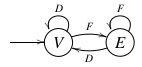
\includegraphics[scale=0.5]{img/skilift.png}

Zutaten: 

\begin{align*}
	A	&= (Q, \Sigma, \delta, q_0, F)  \\
	Q	&= \text{ Zustände} \\
	\Sigma	&= \text{ Alphabet} \\
	\delta	&= \text{ Übergangsfunktion (Pfeile)} \\
	q_0	&\in Q \text{, Startzustand (Initialisierung)} \\
	F	&\subset Q \text{, Akzeptierzustand}
\end{align*}

Zeichenbedeutungen:

$\delta$: Zustand, Zeichen $\rightarrow$ neuer Zustand.

$(q, a) \mapsto q'=\sigma(q,a)$

%$Q \multiply \Sigma \rightarrow^{\sigma} Q$

\subsection{Darstellung mittels Tabelle}

\begin{tabular}{c c}
 & $\Sigma$ \\
$Q$	& $\delta$
\end{tabular}

\subsection{Systematische Rekonstruierung aus der Sprache}

Zustände sind charakterisiert durch "was noch kommen darf"

\begin{align*}
	L(w) = \{v \in \Sigma^\ast | wv \in L \} \\
	\text{Beispiel: } \Sigma = \{a, b \}, L=\{ w \in \Sigma^\ast | |w|_a \text{ gerade}\}
\end{align*}


%TODO: Myhill-Nerode Tabelle mit Zuständen

\begin{align*}
W & L(w) \text{ (was kann angehängt werden)}\\
\varepsilon & L(\varepsilon) = \{v \in \Sigma^\ast | \varepsilon v \in L \} &= L \\
a & L(a) = \{v \in \Sigma^\ast | a v \in L \} &= \{ v \in \Sigma^\ast | |w|_a ungerade \}\\
b & L(b) = \{v \in \Sigma^\ast | b v \in L \} &= L\\
  & L(aa) &= L \\
  & L(ab) &= L(a) \\
  & L(ba) &= L(a) \\
  & L(bb) &= L
\end{align*}

\begin{enumerate}
	\item $L(w)$ ausrechnen: verschiedene $L(w)$ geben $Q$ 
	\item $\sigma: L(w) \rightarrow^a L(wa)$
	\item $q_0: L(\varepsilon) = L$
	\item $L(w)$ ist Akzeptierzustand wenn $\varepsilon \in L(w)$
\end{enumerate}

\subsection{Gleichheit von Automatensprachen feststellen}
	Reduktion auf Minimalautomat M$(A_1)$. Vereinfachung geht, indem zuerst die nicht-Equivalenten zuständige gemäss folgender Liste ausgeschlossen werden:

\begin{enumerate}
	\item Akzeptierzustand $\neq$ Nicht-Akzeptierzustand 
	\item Führt am $m$ Zustände $m$ ein nicht äquivalentes Paar über.
	\item Wiederholung des Algorithmus, bis keine Änderungen mehr auftreten.
	\item Restliche Zustände sind äquivalent.
\end{enumerate}

$\{0^n 1^n | n \geq 0\}$ nicht regulär (Myhill, qualvoll)

\subsubsection{Pumping Lemma}

Alle regulären Sprachen haben die Pumpeigenschaft (aber nicht zwingend umgekehrt).

$L$ regulär $\Rightarrow \exists N$ Punping Length, mit jedes Word $w \in L$ mit $|w| \geq N$ kann zerlegt werden $w=xyz$ mit 
\begin{enumerate}
	\item $|y| > 0$
	\item $|xy| \leq N$
	\item $xy^kz \in L, \forall k \in \mathbb{N}$
\end{enumerate}

\paragraph{Beispiel}

\begin{enumerate}
	\item Annahme: $L = \{ 1^P | p \text{ prim}\}$ ist regulär
	\item ...
\end{enumerate}

\paragraph{Anwendung}

$L=\{0^n1^n|n \geq 0 \}$ ist nicht regulär. Widerspruchsbeweis:

\begin{enumerate}
	\item	Annahme: $L$ ist regulär
	\item	Pumping Lemma: $\exists N$
	\item	Konstruiere $W = 0^N1^N$, $|w| = 2N \geq N$, $w \in L$
	\item	Zerlegung: \\
			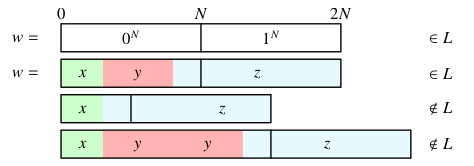
\includegraphics[scale=0.5]{img/pumpinglemma.png}
	\item	Pumpen: $k > 1 \Rightarrow xy^kz$ hat mehr $0$ als $1 \Rightarrow xy^kz \not\in L$ \Lightning $PL: xy^kz \in L$
	\item	Widerspruch: $L$ nicht regulär!
\end{enumerate}

\paragraph{Beispiel}
$\{w \in \varepsilon^\ast | w \text{ ist ein Palindrom }\}$ nicht regulär, $\varepsilon = \{0,1\}$

\begin{enumerate}
	\item	Annahme: $L$ regulär
	\item	PL: $\exists N$
	\item	Konstruiere ein Palindrom: $=0^N1^N1^N0^N$
	\item	Zerlegung: |/x/y/ 0 | 1  |  1 | 0 |
	\item	Pumpe: $k > 1, \Rightarrow xy^kz$ mehr $0$ links als rechts $\Rightarrow \not\in L$ \Lightning
	\item	Widerspruch: $L$ ist nicht regulär
\end{enumerate}

\subsection{Nicht deterministische Automaten}

\[
 \lambda : Q \times (\Sigma \cup \{\varepsilon\}) \rightarrow P(Q)
\]

$\cup \{\varepsilon\}$ ermöglich Sprünge; es können "Pfeile" weggelassen werden und es können mehrere Pfeile für den gleichen Buchstaben geben.

\paragraph{Beispiel} $L=\{ w \in \sigma^\ast | w \text{ beginnt und endet mit } 0\}$

%TODO: Graphik: ->kreis -0->kreis(selbstverweis für 0,1) -0-> doppelkreis
%\begin{tikzpicture}[>=stealth',auto,node distance=2cm]
%TODO!!!
%\node[initial,state] (q0) {$q_0$};
%\node[state] (q1) [right of=q0] {$q_1$};
%\node[state] (q2) [right of=q1] {$q_2$};
%\node[state] (q3) [right of=q2] {$q_3$};
%\node[state, accepting] (q4) [right of=q3] {$q_4$};
%
%\path[->]
%(q0)	edge [bend left]	node {a} (q1)
%(q1)	edge [bend left]	node {a} (q2)
%(q2)	edge [loop above]	node {a} (q2)
%edge [bend left]	node {b} (q3)
%(q3)	edge [bend left]	node {b} (q4)
%edge [bend left]	node {a} (q2)
%(q4)	edge [loop below]	node {b} (q4)
%edge [bend left]	node {a} (q2);     
%\end{tikzpicture}

$w$ wird akzeptiert $\equiv \exists$  es gibt einen Weg, der auf einen Akzeptierzustand führt.

Aus so einem Graphen lässt sich immer einen endlichen Automaten konstruieren.


\subsection{$\text{NEA}_\varepsilon \to \text{DEA}$}

$\varepsilon$-Übergänge sind "gratis", d.h. verbrauchen kein Zeichen.


-> Alle Zustände / Kombinationen von Zuständen aufzeichnen
-> Alle Übergänge durchprobieren


\subsection{Mengenoperationen}
\subsubsection{Komplement}

Endzustände Streichen, alle anderen Zustände in Endzustände umwandeln.


\subsection{Reguläre Ausdrücke}

Ziel: Notation für reguläre Spraceh "reguläre Ausdrücke": $r$

\[
	L(r) = \{ w \in \Sigma^\ast | \text{ Wort } w \text{ passt auf den reg. Ausdruck } r\}
\]

Bausteine: primitiven reg. Ausrücke (Wörter mit höchstens 1 Zeichen)

\begin{tabular}{ l l}
	a & steht für $L(a) = \{ a \}$ \\
	. & steht für $L(.) = \{a,b,c\} = \{ w \ in \Sigma ^ \ast | |w| = 1 \}$\\
	$[0-9]$ & steht für $L([0-9])=\{w \in \{ 0, 1, ..., 9\}| |w| = 1 \}$\\
	$\varepsilon$ (leeres Wort) & steht für $L("") = \{ \varepsilon \}$
\end{tabular}

\subsubsection{Reguläre Operationen}

\begin{align*}
\text{Verkettung: } & L(r_1), L(r_2) \Rightarrow L(r_1,r_2) = L(r_1)L(r_2) \\
\text{Alternative: }& L(r_1),L(r_2) \Rightarrow L(r_1|r_2) = L(r_1) \cup L(r_2) \\
\text{*-Operation: }& L(r) \Rightarrow L(r^\ast) = L(r)^\ast
\end{align*}

\paragraph{Beispiel}

	\emph{(0 | (|-)[1-9][0-9]*)}  alternative Schreibweise \emph{-? r?} \\
	\emph{[0-9]+\.[0-9]+\.[0-9]+\.[0-9]}


\subsubsection{Umwandlung Automat / Ausdruck}
Umwandlung in einen Automat mit Startzustand $S$, einem Übergang $r$ und einen Akzepttierzustand $A$

Vorgehen, um einen Automaten in einen Ausdruck umzuwandeln:

\begin{itemize}
	\item Startzustand un Endzustand mittels $\varepsilon$-Übergängen hinzufügen.
	\item Zwischenzustände entfernen.
\end{itemize}

\section{Kontextfreie Grammatik}


Kann im Gegensatz zu Regulärer Sprache z.B. $\{0^n1^n | n \geq 0 \}$ darstellen. Dazu gehören alle moderne Programmiersprachen.

\paragraph{Beispiel Klammern $(()())$}

Mit Klammern können wir:

\begin{enumerate}
	\item $\varepsilon$ \hfill $A \to \varepsilon$
	\item Verketten \hfill $A \to AA$
	\item «Einklammern» \hfill $A \to (A)$
\end{enumerate}

diese 3 Regeln produzieren einen Klammerausdruck:
\[
	A \to (A) \to (AA) \to ((A)A) \to ((A)(A)) \to (()(A)) \to (()())
\]

\subsection{Definitionen}

\[
	G = (V, \Sigma, R, S)
\]

\begin{description}
	\item[$V$] \hfill \\
		Variable, Platzhalter für (Teil-)Ausdrücke
	\item[$\Sigma$] \hfill \\
		Terminalsymbole (Alphabet)
	\item[$R$] \hfill \\
		Regeln: $A \to BCx$ Zeichenkette von Variablen und Terminalsymbolen
	\item[$S$] \hfill \\
		Startvariable $S \in V$
\end{description}

Wir arbeiten \emph{Kontextfrei}, d.h. auf der linken Seite steht nur eine Variable.

Definition: $L$ kontextfrei $\Leftrightarrow L(G)  L$, $G$ kontextfreie Grammatik.


\paragraph{Beispiel I} \hfill \\
\[
	(\{A\}, \{(,)\}, \{A \to \varepsilon, A \to AA, A \to (A)\}, A)
\]

\paragraph{Beispiel: II}

Natürliche Zahlen ohne führende Nullen
\begin{align*}
	\text{Zahl} &\to \text{ziffer} \\
	\text{} &\to \text{ziffer} \\
	\text{ziffernfolge} &\to \text{ziffer} \\
	\text{} &\to \text{ziffernfolge ziffer}
\end{align*}

\begin{align*}
	\text{nichtnullziffer} &\to 1 | 2 | ... | 9 \\
	\text{ziffern} &\to 0 | \text{nichtnulziffer}
\end{align*}


\subsubsection{Notation}

$A \xRightarrow{\ast} w$

$w$ ensteht aus $A$ durch Regelanwendung. $w$ ist aus $A$ ableitbar.

\subsection{Voraussagbare Effizienz / Chomsky-Normalform}
Schlechte Ansätze:
\begin{itemize}
	\item Start auf der rechten Seite: Beliebig oft Schachteln.
	\item $\varepsilon$-Regeln: $A \to \varepsilon$ (Arbeit verrichten)
	\item Unit Rules: $A \to B$ (Endlosschleifen)
	\item $A \to u_1,u_2,...,u_n$ (Wortexplosionen)
\end{itemize}

Kochbuch guter Ansatz:

\begin{itemize}
	\item Startvariable nicht rechts
	\item $S \to \varepsilon$ als einzige $\varepsilon$-Regel
	\item Keine Unit Rules
	\item Nur Regeln der Form $A \to BC$ und $A \to a$
\end{itemize}

Forderung: $G$ heisst $m$ Chomsky-Normalform (CNF). In der CNF Braucht die Konstruktion von Wörtern $2 \cdot |w| -1$ Schritte.

 \subsection{Effizienter Parse-Algorithmus finden}
 
%TODO: Pseudo Algorythmus aus Script übernehmen

\subsection{Stackautomaten}

\begin{align*}
P &= (Q, \Sigma, \Gamma, \delta, q_0, F) \\
\Gamma & \\
\delta&: Q \times \Sigma_\varepsilon \times \Gamma_\varepsilon \to P(Q \times \Gamma) \\
\Sigma_\varepsilon &= \Sigma \cup \{ \varepsilon \}
\end{align*}

\subsubsection{Grammatik $\rightarrow$ Stackautomat}

\paragraph{Beispiel}

\[
L = \{ 0^n 1^n | n \geq 0 \}
\]

Grammatik:
\begin{align*}
S &\rightarrow 0S1 \\
  &\rightarrow \varepsilon
\end{align*}

Idee: Zwischenresultate der Produktionsregeln auf den Stack. Dies führt zur Konstruktion eines Stackautomaten, welcher immer vorzu matched, ob der Input der Sprache entspricht.



Am Anfang: $\varepsilon, \varepsilon \to \$; \varepsilon, \varepsilon \to S$


Von und zum Zentralen Punkt: 
\begin{align*}
A \to BC & \varepsilon, A \to c, \varepsilon, \varepsilon \to B \\
A \to a & \varepsilon, A \to a \\
S \to \varepsilon & \varepsilon, S \to \varepsilon \\
a, a \to \varepsilon & \text{(für jedes Terminalsymbol)} \\
\text{Am Ende:} & \varepsilon, \$ \to \varepsilon 
\end{align*}

\subsubsection{Stackautomat $\to$ Grammatik}

\begin{itemize}
	 \item Nur 1 Akzeptierzustand
	 \item Stack leer beim Akzeptieren (wegschmeissen von allem verbliebenem.
	 \item Bei jedem Übergang genau 1 Zeichen auf den Stack oder 1 Zeichen vom Stack (ersetzen von Zeichen nur über Umweg $\varepsilon$ möglich)
\end{itemize}

$w$ akzeptiert: es gibt einen Pfad durch den Stackautomaten von $q_0$ zu $q'_a$, Stack leer.

\begin{tabular}{l l l r}
	Startvariable: & $S$&$=A_{q_0 q'_a}$ &Startzustand zu Endzustand \\
	& $A_{pq}$&$= $ Wörter, die $p$ in $q$ überführen mit leerem Stack.
\end{tabular}

\paragraph{Spezialfälle}

Stack kommt irgendwann zwischendurch bei $r$ auf 0 $\Rightarrow A_{pq} \to A_{pr} A_{rq}$

Ein Wort vom Anfang des Stacks wird am Ende erst wieder abgebaut: $\Rightarrow A_{pq} \to a A_{rs} b$

\subsection{Backus-Naur-Form}

Standard für die Formulierung von Grammatiken.

Extended BNF: Wiederholungen, Kommentare etc.


\subsection{Pumping Lemma für kontextfreie Sprachen}

$L$ kontextfrei $\Rightarrow \exists N \text{ pumping length }$

N muss genug gross sein, damit eine Variable zweimal verwendet wird.

\[
	w \ in L \text{ mit } |w| \geq N \Rightarrow w = uvxyz
\]
mit:
\begin{itemize}
	\item $|vy| > 0$
	\item $|vxy | \leq N$
	\item $uv^ky^kz \in L$, $\forall k$
\end{itemize}

Warum? $L$ kontextfrei: $\Rightarrow$ $G$ Grammatik von $L$, in CNF.

%TODO: GRAFIK 1



\paragraph{Beispiel}

\[
	\{a^n b^n c^n | n \geq 0 \} \text{ nicht kontextfrei?}
\]

\begin{enumerate}
	\item Annahme: $L$ kontextfrei
	\item $\exists N$
	\item $w = a^N b^N c^N$, mit $|w| = 3N$
	\item Unterteilung: %TODO: GRAFIK 2
	\item Anzahl von 2 Buchstaben wird erhöht, aber nicht vom dritten!
		$\rightarrow$ Pumpen führt aus L hinaus! Darum:
	\item $\Rightarrow L$ ist nicht kontextfrei
\end{enumerate}

\section{Turing-maschinen}

Speicher: Beidseitig unendlich langes Band aus Speicherzellen. Prefilled with Blanks: ␣.

Universelle Turing Maschine: Programm + Daten auf einem Band.

Endlicher Automat der ''entscheidet'' was mit dem Inhalt an der Speicherzelle geschehen soll und Bewegung um 1 Feld Links oder 1 Feld Rechts.

%TODO: Insert G1

Läuft selbständig!

\paragraph{Definition}
\begin{description}
	\item[Q] Zustände Endlicher Automat
	\item[$\Sigma$]alphabet
	\item [$\Gamma$] Initialisierung des Bandes mit speziellem Blank ␣
	\item[$\delta$] Zustandsübergänge
	\item[$q_0$] Startzustand
	\item[$q_{accept}$] Alles Bestens, finito
	\item[$q_{reject}$] Nicht gut, finito
\end{description}

\[
	M=(Q, \Sigma, \Gamma, \delta, q_0, q_{accept}, q_{reject})
\]
\[
	\delta: Q \times \Gamma \rightarrow Q \times \Gamma \times \{L, R\}
\]

%TODO: Insert G2

\begin{enumerate}
	\item $w$ auf das Band schreiben
	\item Lesekopf auf erstes Zeichen
	\item $\rightarrow q_{accept} \Rightarrow w$ wird akzeptiert
\end{enumerate}

Sprache: $L(M) = \{w \in \Sigma^\ast | M \text{ endet in } q_{accept} \}$
von M \emph{erkannte Sprache}.

\paragraph{Beispiel} eines Automaten mit ungerader Länge.

\[
	L = \left\{w \in \Sigma^\ast \left| \left|w\right| ungerade \right.\right\}
\]

%TODO: Insert G3

Diese Turing-Maschine hält auf jeden Input an; dies wird als Entscheider bezeichnet.

\paragraph{Beispiel 2} Korrekte Klammerausdrücke

\[
	\Sigma = \{(,)\}, L = \{w \in \Sigma^\ast | w \text{ korrekte Klammerausdrücke } \}
\]

z.B: (()())


\subsection{Varianten von Turing-Maschinen}

\subsubsection{Mehrspurige TM}

Maschine liest immer mehrere Spuren von $\Gamma$-Werten aus; eigentlich also eine gewöhnliche TM mit Bandalphabet $\Gamma^3$, einfach etwas Schneller da sie 3 Wörter pro Durchlauf verarbeitet.

\subsection{Mehrere Bänder}

Schneller, da zwei unabhängige ''Leseköpfe''. Das lässt sich mit zwei zusätzliche Bändern, welche den aktuellen Ort markiert, auf einer klassischen Turing-Maschine realisieren.

\subsection{Es reicht: $\Gamma = \{ 0, 1, \text{␣}\}$ für jeden Computer}

Wie: längere Zeichen werden durch Binärstrings codiert. Mit (endlich) vielen Zuständen kann so ein beliebiger Computer Simuliert werden.


\subsection{Begriffe}

\begin{description}
	\item[Turing erkennbar] \hfill \\
		$L$ heisst Turing erkennbar $\equiv \exists TM$ M mit $L(M)=L$
	\item[Turing entscheidbar] \hfill \\
		$L$ heisst Turing entscheidbar $\equiv \exists TM$ M, Enscheider $L(M)=L$ zum Enscheiden, ob es eine Endlosschleife hat oder nicht.
	\item[Aufzähler] \hfill \\
		TM mit Drucker, schreibt alle Wörter der Sprache auf den Drucker. \\
		eine Sprache $L$ ist aufzählbar $\equiv$ $L$ ist Turing erkennbar.
\end{description}

%TODO: Insert G5

\subsection{Berechnung}

TM $M$

\begin{enumerate}
	\item Input auf Band
	\item TM laufen lassen
	\item Resultat ist auf Band
\end{enumerate}

\subsubsection{Die Mächtigkeit von Mengen}

kann mit einer bijektiven Abbildung von Menge $A$ auf $B$ gezählt werden $\Rightarrow |A| =  |B|$

Beispiel: Hotel unendlich hat Zimmernummern $\mathbb{N}$


$\mathbb{N}$ ist abzählbar unendlich. D.h.: Die Objekte können ''durchnummeriert'' werden. 

Vereinigungen mit abzählbar unendlichen Mengen sind abzählbar unendlich ($A \cup B =$ abzählbar unendlich), $A \times B$ auch.

\begin{description}
	\item[$\mathbb{N}$] abz. unendlich
	\item[$\mathbb{Z}$] abz. unendlich.
	
	\item[$\mathbb{Q}$] abz. unendlich
	\item[$\mathbb{R}$] überabzählbar.
\end{description}


\subsubsection{Beweis, $\mathbb{R}$ überabzählbar}

Annahme: $\mathbb{R}$ ist abz. $\infty \Rightarrow$ List der reelen Zahlen, kann also mit Zahlen aus $\mathbb{N}$ in Verbindung gebracht werden:

\begin{tabular}{l l}
	0 & 0.|1|11111111.... \\
	1 & 0.3|1|415926535... \\
	2 & 0.23|4|56721234... \\
	3 & 0.1414|2|135... \\
	... & ...
\end{tabular}

Es gibt eine Zahl, die in der Liste nicht vorkommt: $0.22253...$ immer was anderes als bei den Zahlen oben an der jeweiligen steht.

Widerspruch: es gibt eine Zahl, welche nicht in der Liste steht.


\subsubsection{Was kann man berechnen?}

Berechenbar sind alle Sprachen, welche Turing-erkennbar sind.

Antwort durch zählen: leider gibt es unendlich viele. 

$\Sigma^\ast$ abzählbar, genau wie Turing Maschinen, Programme etc, da diese abgezählt werden können.

Die Sprachen $P(\Sigma^\ast)$ ist überabzählbar. Es gibt viel mehr Sprachen als es Programme gibt.

\subsection{Entscheidbarkeit}

Sprache $L$ heisst entscheidbar, wenn: $\exists$ Turing Maschine $M$ mit $L(M) = L$; $M$ ist Entscheidbar: $M$ hält auf jeden Input.

Sprache $L$ heisst Turing erkennbar, wenn: $\exists$ TM $M$ mit $L(M)=L$

\[
	\text{Entscheidbar} \subset \text{Turing erkennbar} \subset P(\Sigma^\ast)
\]


\subsubsection{Beispiele}
	
	
\paragraph{Hilbertsches Problem}
\[
	x^n + y^n = z^n
\]

ist nicht für alle $n$ eindeutig entscheidbar.

Die Gleichheit von zwei Ausdrücke sind ein nicht entscheidbares Problem.

 \paragraph{Beispiel 2}
 
 $L$ regulär $\Rightarrow$ $L$ entscheidbar
 
 $L$ entscheidbar $\Leftrightarrow \exists$ Entscheider $M$, $L(M) = L$
 
 $L$ regulär $\Leftrightarrow \exists$ DEA $A$ mit $L(A) = L$
 
 Entscheider für $L$: Simuliere DEA $A$ auf Input-Wort mit TM $M$.
 
 Falls $A$ akzeptiert $\rightarrow q_\text{accept}$, falls $A$ nicht akzeptiert $\rightarrow q_\text{reject}$
 
 $\Rightarrow L$ ist daher entscheidbar!
 
 \paragraph{Beispiel 3}
 
 $L$ kontextfrei $\xRightarrow ? L$ entscheidbar
 
 $L$ kontextfrei $\Rightarrow \exists G$ Grammatik $L(G)=L$
 
 Entscheider für $L$: CYK-Algorithmus implementieren, entscheidet in $O(|w|^3)$, ob $w \in L = K(G)$
 
\subsubsection{Übersetzung in Sprachproblem}
 \paragraph{Entscheidungsprobleme für Reguläre Sprachen}
 
 <$B,w$> (Codierung von $B$ und $w$)
 
 \begin{tabular}{l l}
 Frage: &Kann man mit einem Programm entscheiden, ob ein DEA $B$ ein Wort $w$ akzeptiert. \\
 Input: &$B$, $w$ \\ 
 Output: &ja|nein: $w \in L(B)$ \\
Sprachproblem: & $ A_\text{DEA} = \{ <B,w> | B \text{ ein DEA, } w \in \Sigma^\ast, w \in L(B) \} $ \\
& Dieses Problem nennt man Akzeptanzproblem für DEAs. \\
Antwort: &Programm mit Input $<B,w>$, \\
&1. $B$ als regulärer Ausruck codieren \\
&2. verwende regex-Engine, die enscheidet, ob $w \in L(B)$
\end{tabular}

\paragraph{DEA II} \hfill \\


\begin{tabular}{l l}
Frage: &Kann man mit einem Programm entscheiden, ob für einen beliebigen DEA $B$ gilt: \\
& $L(B) = \emptyset$? \\
Input:&$B$, ein DEA \\
Putput: &ja|nein \\
Sprachproblem: & Ist $E_\text{DEA} = \{<B>|B \text{ ein DEA, } L(B) = \emptyset$ entscheidbar? \\
Antwort: & 1. Startzustand Markieren \\
		&2. von markierten Zuständen aus erreichbare Zustände markieren. \\
		&   (wiederhole, solange neue Markierungen) \\
		& Akzeptier-Zustand markiert? ja $\rightarrow q_\text{reject}$, $\rightarrow q_\text{accept}$ \\
Antwort 2:	&1. Minimalautomaten herstellen: $B =^? \rightarrow O\leftrightarrow$ \\
			& ja $\rightarrow q_\text{accept}$, nein $\rightarrow q_\text{reject}$
\end{tabular}

\paragraph{Zwei Reguläre Sprachen gleich?} \hfill \\

\begin{tabular}{l l}
	Frage: &Kann man mit einem Programm entscheiden, ob zwei reguläre Sprachen gleich sind? \\
	Input: &$B_1, B_2$ DEAs \\
	Output: &ja|nein: $L(B_1) = L(B_2)$ \\
	Sprachenproblem: &ist $EQ_\text{DEA} = \{<B_1, B_2> | B_i \text{ sind DEAs}, L(B_1) = L(B_2)\}$ \\
		& entscheidbar? Geichheitsproblem für DEAs. \\
	Antwort: &1. Minimalautomat($B_1$) $=^?$ Minimalautomat($B_2$): \\
			 &   ja $\rightarrow q_\text{accept}$, nein $\rightarrow q_\text{reject}$ \\
	Antwort 2: & $(L(B_1) \cup L(B_2)) \setminus (L(B_1) \cap L(B_2)) = L(B_1) \bigtriangleup L(B_2) =^? \emptyset$ \\
	&1.	Endlicher Automat für: $L(B_1) \bigtriangleup L(B_2)$ mit Mengenoperationen \\
	&2.	Entscheider für $E_\text{DEA}$ darauf anwenden.	
\end{tabular} 
 
$\bigtriangleup$ = Symmetrische Differenz

\subsubsection{Entscheidungsprobleme für CFLs}

%Siehe script 6.1.3

Antwort: 1. $G$ in CNF $\rightarrow G'$ \\
		 2. CYK-Alg. auf $G'$ und $w$ anwenden $\rightarrow$ ja|nein



\subsubsection{Bisher untersuchte Probleme entscheidbar?}

\begin{tabu}{l X}
	Frage: &Kann man mit einem Programm entscheiden, ob eine TM $M$ ein Wort $w$ akzeptiert \\
	Input: &$M, w$\\
	Output: &ja / nein\\
	Sprachproblem: & $A_\text{TM}=\{\left<M,w\right>  M \text{ eine TM, } w \in \Sigma^\ast, w \in L(M) \}$ entscheidbar?\\
	Antwort: &nein!
\end{tabu}

Beweis: (Widerspruchsbeweis)

\begin{enumerate}
	\item	Annahme: Es gibt ein Enscheider $H$ für $A_\text{TM}$
	\item	$H(M,w) = \begin{cases}
			q_\text{accept}\\
			q_\text{reject}
		\end{cases}$
		m akzeptiert w / m verwirtf w \\
	\item	Neue TM D: auf Input $<M>$ \begin{enumerate}
			\item $H$ auf $\left<M,\left<M\right>\right>$ laufen lassen
			\item $q_\text{accept} : \rightarrow q_\text{reject}$
			\item $q_\text{reject} : \rightarrow q_\text{accept}$
		\end{enumerate}
		Analyse von D: \[
			D(\left<M\right>) \begin{cases}
			q_\text{accept} & M \text{ verwirft } <M>\\
			q_\text{reject} & M \text{ akzeptiert } <M>\\
			\end{cases}
		\]
	\item Wähle: $M=D$: \[
			\begin{cases}
			q_\text{accept}, D \text{ akzeptiert } <D> & D \text{ verwirft } <D>\\
			q_\text{reject}, D \text{ verwirft } <D> & D \text{ akzeptiert } <D>\\
			\end{cases}
		\]
	\item	$\Rightarrow$ Annahme falsch $\Rightarrow \nexists H \Rightarrow A_\text{TM}$ nicht entscheidbar!
\end{enumerate}


\subsubsection{Spezielles Halteproblem: nicht entscheidbar.}

Wichtig: Das Haltetheorem zeigt, dass etwas nicht entscheidbar ist.

\begin{tabu}{l X}
	Frage: &... ob eine TM $M$ auf $\varepsilon$ anhält?\\
	Input: & $M$\\
	Output: & ja|nein\\
	Sprachproblem: &$ \{\left<M\right>|M \text{ TM, } M \text{ hält auf Input } \varepsilon$\\
	Antwort: &Ist dies entscheidbar? Nein!
\end{tabu}

\begin{enumerate}
	\item Annahme: es gibt einen Entscheider $H$ für Halte TM. \[
		H(M) \begin{cases}
			q_\text{accept} & M \text{ hält.}\\
			q_\text{reject} & M \text{ hält nicht.}
		\end{cases}
	\]
	\item	Input: $\left<M,w\right> \longrightarrow$ neues Programm $M'$: \begin{enumerate}
			\item lasse $M$ auf $N$ laufen
			\item $q_\text{accept}: \rightarrow q_\text{accept}$
			\item $q_\text{reject}:$ Endlosschleife
		\end{enumerate}
		$M'$ hält, wenn $H(M') = q_\text{accept}$
	
\end{enumerate}

$\Rightarrow \left<M,w\right> \longrightarrow M' \xrightarrow{ H } \begin{cases}
	q_\text{accept} & \text{ entscheidet } A_\text{TM}\\
	q_\text{reject} & \text{ entscheidet } A_\text{TM}\\
\end{cases}$ \Lightning

Widerspruch!


\subsubsection{Satz von Rice}

Beispiel: $HALT_{TM} = \{ \left<M,w\right> | M \text{ eine TM, } M \text{ hält auf Input } w \}$

nicht entscheidbar.

Beweis:

\begin{tabu}{l X}
	$A_{TM}$ &$\xrightarrow{f} HALT_{TM}$ \\
	$\left<M,w\right>$ &$\rightarrow \left<S,w\right>$ \\
	$M$ akzeptiert $w$ & $\rightarrow$ $S$ hält auf Input $w$: \begin{enumerate}
		\item $M$ auf Input $w$ laufen lassen
		\item $q_\text{accept} \rightarrow q_\text{accept}$
		\item $q_\text{reject} \rightarrow$ Endlosschleife
		\end{enumerate}
\end{tabu}

Abbildung $A_{TM} \leq HALT_{TM}$ (''leichter zu entscheiden als'')

$w \in A \Rightarrow f(w) \in B$. $f$ ist berechenbar: $\Rightarrow f: A \leq B$

\begin{tabu}{l l X}
Folgerung: &$B$ entscheidbar&$\Rightarrow A$ entscheidbar \\
	&$A$ nicht entscheidbar &$\Rightarrow B$ nicht enscheidbar
\end{tabu}

Somit wurde der Schwierigkeitsgrad des Problems ermittelt.

\subsubsection{Beispiel 2}

Das Komplementär (Gegenteil) eines Problems ist auch nicht entscheidbar, wenn das Problem nicht entscheidbar ist.

Beweis durch Reduktion $A_{TM} \leq \overline{E}_{TM}$:

\begin{tabu}{l X}
	$\left<M,w\right> $ &$\rightarrow \left<S\right>$ \\
	$M$ akzeptiert $w$ &$\rightarrow L(S) $ nicht leer. \\
	& Konkret: $L(S) = \{w\}$ \\
	& $S$ auf Input $u$ abbilden: \begin{enumerate}
		\item $u \neq w \rightarrow q_\text{reject}$
		\item $M$ auf $w$ laufen lassen
		\item $q_\text{accept} \rightarrow q_\text{accept}$
		\item sonst $ \rightarrow q_\text{reject}$
		\end{enumerate}
\end{tabu}

$P$ eine Eigenschaft von Turing erkennbarer Sprache.
\[
P_{TM} = \{\left<M\right> | L(M) \text{ hat eigenschaft } P \}
\]
\[
\overline{P}_{TM} = \{\left<M\right> | L(M) \text{ hat eigenschaft } P \text{ nicht.}\}
\]

\begin{tabu}{l X}
	Reduktion: &$A_{TM} \leq \overline{P}_{TM}$; Annahme: $\emptyset$ hat Eigenschaft.\\
	& $\left<M,w\right> \rightarrow \left<S\right>$ \\
	& $M$ akzeptiert $w$ $\rightarrow$ $L(S)$ hat Eigenschaft $P$ nicht. Konkret: $L(S) = L_1$ (hat $P$ nicht).\\
	& $S$ auf Input $u$ \begin{enumerate}
		\item $M_1$ auf $u$ laufen lassen: $q_\text{reject} \rightarrow q_\text{reject}$
		\item $M$ auf $w$ laufen lassen
		\item $q_\text{accept} \rightarrow q_\text{accept}$
		\item sonst $\rightarrow q_\text{reject}$
	\end{enumerate}
	Was heisst: $L(S) = L_1$ hat $P$ nicht; $L(S) = \emptyset$ hat $P$.
\end{tabu}


\subsubsection{Beispiel 3: Regulär?}


\begin{tabu}{l X}

Problem: &$REGULAR_{TM} = \{ \left<M\right> | \text{ Meine TM, } L(M) \text{ regulär }\}$ nicht entscheidbar. \\
& $\overline{REGULAR}_{TM} = \{\left<M\right> | \text{ Meine TM, } L(M) \text{ nicht regulär} \}$ nicht entscheidbar.	\\
Reduktion: & $A_{TM} \leq \overline{REUGLAR}_{TM}$ \\
	&$\left<M,w\right> \rightarrow \left<S\right>$ \\
	$M$ akzeptiert w &$\rightarrow L(S)$ nicht regulär, konkret: $L(S) = \{0^n1^n | n \geq 0 \}$ \\
$w \not\in L(M)$ &$\rightarrow$, konkret: $L(S) = \emptyset$ \\
& $S$ auf Input $u$: \begin{enumerate}
		\item $u$ nicht $0^n1^n \rightarrow q_\text{reject}$
		\item $M$ auf $w$ laufen lassen
		\item $q_\text{accept} \rightarrow q_\text{accept}$
		\item sonst $\rightarrow q_\text{reject}$
	\end{enumerate}
\end{tabu}

\subsection{Satz von Rice?}

$P$ Eigenschaft, zwei Beispiele: $L_0 \rightarrow$ hat $P$, $L_1 \rightarrow$ hat $P$ nicht. Dies nennt man nicht triviale Eigenschaften (nicht offensichtlich).

Dann ist $P_{TM}$ nicht entscheidbar!

\paragraph{Beispiel:}

\begin{enumerate}
	\item $P=E$; ''Sprache ist leer''\\
		$L_0 = \emptyset$ \\
		$L_1 = \{w\}$ \\
		Weil Turing erkennbar $\Rightarrow E_{TM}$ nicht entscheidbar (Rice)
	\item $P = CFL$ ''Sprache ist kontextfrei'' \\
		$L_0 = \emptyset$ \\
		$L_1 = \{0^n1^n2^n | n \geq 0\}$ \\
		Turing erkennbar $\xRightarrow{\text{Rice}} CFL_{TM}$ nicht entscheidbar.
	\item $P = ALL$; ''Sprache ist $\Sigma^\ast$'' \\
		$L_0 = \emptyset$ \\
		$L_1 = \Sigma^\ast$ \\
		Turing erkennbar $\xRightarrow{\text{Rice}} ALL_{TM}$ nicht erkennbar.
	\item $P = PRIMES$; ''Sprache besteht genau aus den Primzahlen'' \\
		$L_0 = \{ 42 \}$ \\
		$L_1 = \{Primzahlen\} = \mathbb{P}$ \\
		Turing erkennbar $\xRightarrow{\text{Rice}} PRIMES_{TM}$ nicht entscheidbar.
	\item $P = SPEZ$; ''Sprache erfüllt eine Spezifikation'' \\
		$L_0 = \emptyset$ \\
		$L_1 = \{...\text{korrekte Sourcecodes}...\}$ \\
		Turing erkennbar $\xRightarrow{\text{Rice}} SPEZ_{TM}$ nicht entscheidbar (kann Compiler nicht automatisch auf Validität testen.
\end{enumerate}

\subsubsection{Noch ein Beispiel Reduktion}


Beispiel für Reduktion: $EQ_{TM} = \{\left<M_1,M_2\right> | M_i TMs, L(M_1) = L(M_2) \}$

$E_{TM} \rightarrow$ maschine ohne akzeptiertes Wort; nicht entscheidbar.

$M_\emptyset$ Maschine, die nichts akzeptiert.

$E_{TM} \longrightarrow EQ_{TM} $

$ \left<M\right> \longrightarrow \left<M, M_\emptyset\right>$

$\Rightarrow E_M \leq EQ_{TM} \Rightarrow EQ_{TM} $ nicht entscheidbar.

$L(M) \text{ leer } \Leftrightarrow L(M) = L(\underbracket{TM \text{, die nichts akzeptiert }}_{M_\emptyset})$

\section{Komplexitätstheorie}

\emph{Erweitern entscheidbar oder nicht entscheidbar (''vernünftiger Zeit'')}

Probleme die in ''vernünftiger Zeit'' lösbar sind.

\begin{tabu}{l X}
	Ziel: & Unterscheiden zwischen in ''vernünftiger Zeit'' lösbarer Probleme und ''langsamer'' Probleme \\
	vernünftig &$\rightarrow$ Klasse P \\
	''unvernünftig'' &$\rightarrow$ Klasse NP \\
	Mass für laufzeit: & \begin{enumerate}
			\item	unabhängig von Hardware
			\item	abhängig von der Problemgrösse: $n = $ Länge des Inputwortes.
			\item	Worst case
			\item	''bester Algorithmus''
		\end{enumerate}
\end{tabu}


\subsection{Hardwareabhängigkeit}

\paragraph{Simulation einer mehrspurigen TM} auf einer Standard-TM.


$1$ Schritt $\longrightarrow c$ Schritte. \\
\begin{tabu}{l l l l}
Laufzeit auf Input $w$ & $t(w)$ &$\longrightarrow c \cdot t(w)$ & $O(t(w))$ ändert nicht \\
Mass für laufzeit: &$t(n) = \max t(w)$; $|w| = n$ & $\longrightarrow O(T(n))$ 
\end{tabu}

\paragraph{Simulation einer Mehrband-TM} auf einer Standard-TM

1 Schritt $\longrightarrow$ Anzahl beschriebenen Zellen $\leq t(n) \approx O(t(n))$

$t(n)$ Schritte: $\longrightarrow$ $O(T(n)^2)$

Laufzeitmass muss unabhängig sein von Exponenten ($^2$).

\paragraph{Conclusion:} \hfill \\
Laufzeit ist Polynomiell, wenn $t(n) = O(n^k)$ ist.

Klasse P: Sprachen, die in polynommieller Laufzeit entschieden werden können.



Die Abgrenzung zwischen Polynomiell und exponentiell ist ''schwierig''
$\underbracket{1 + n + \frac{n^2}{2!} + \frac{n^3}{3!} ... }_{\text{polynomiell}}= \underbracket{e^n}_{\mathrlap{\text{exponentiell}}}$

$\Rightarrow$ Unterscheidung muss Feature er TM verwenden: Nicht-deterministische TM.

\subsection{Laufzeit}

\begin{tabu}{l X}
	Ziel: &Vergleich von Problemstellungen nach Laufzeit \\
		  & \begin{itemize}
			  	\item Hardwareunabhängig
			  	\item Worst Case
			  	\item In Abhängigkeit von Input-Länge: $n=|w|$
		  	\end{itemize}
		  	Wegen der Worst-Case-Forderung: $t(n) = max(t(w))$

			Polynomielle laufzeit: $\Rightarrow t(n) = O(n^k)$
			
			Klasse $P$: Sprachen die in polynomieller Zeit enschieden werden können.
\end{tabu}


\subsubsection{Beispiel}

Ist $L$ in $P$? Was tun? $\longrightarrow$ Algo mit polynomieller Laufzeit.

\paragraph{Beispiel 1} $\text{PATH} = \{ \left< G, s, t \right> | G \text{ ein gerichtetter Graph, } \exists \text{ Pfad von } s \text{ nach } t\} \in P$

Vorgehen: immer erreichbare Knoten markieren, um herauszufinden, ob ein Weg existiert: Laufzeit: Anzahl Iterationen $\leq$ Anzahl Knoten $\leq n$  
mit (Anzahl Knoten)$^2$ Tests $\leq n^2$ $\longrightarrow O(n^3)9$
	
\paragraph{Beispiel 2} $\text{RELPRIME} = \{ \left<a,b\right> | a, b \in \mathbb{Z}, \text{ teilerfremd} \} \in P$

($a$, $b$ Binärzahlen).

Euklid: In jedem Schritt nimmt die Länge der Zahlen $a$ und $b$ um ein Bit ab.

$\Rightarrow$ Laufzeit $\leq$ Bitzahl des Input $\leq O(\log_2{a} + \log_2{b}) = O(n^1)$


\subsection{Klasse NP}

\emph{Definition:} Sprachen, die sich in polynomieller Zeit von einer \textbf{nicht deterministischen} Turing Maschine entscheiden lässt.

$P \subset NP$

\subsubsection{Was ist eine nicht deterministische TM?}
\[
	M= (Q, \Sigma, \Gamma, \delta, q_0, q_\text{accept}, q_\text{reject})
\]
\[
	\sigma: Q \times \Gamma \longrightarrow P(Q \times \Gamma \times \{L,R\})
\]
Es gibt mehrere Möglichkeiten, wie weitergerechnet wird.

\subsubsection{Was akzeptiert eine n.d. TM?}

$\Leftrightarrow$ es gibt eine Berechnung, die zu $q_\text{accept}$ führt.

\subsubsection{Was ist ein Entscheider?}

Terminiert jede Berechnung?


\subsubsection{Wie wird die Laufzeit gemessen?}

Maximum aller möglichen Berechnungswege.

\subsubsection{Wie lässt sich eine n.d. TM simulieren?}

$M$ nicht deterministische TM. $\longrightarrow$ auf Standard-TM simulieren.


\begin{itemize}
	\item Zu einem Input $|w| = n$ ist jede Berechnung $\leq t(n)$
	\item Anzahl Berechnungen (worst case): in jedem Schritt gibt es $\leq c$ Wahlmöglichkeiten. Total: $c^{t(n)}$ Berechnungswege.
\end{itemize}

Insgesamt: \[
	c^{t(n)} \cdot t(n) = 2^{t(n) \log_2 c + \log_2(t(n)} = 2^{O(t(n))}
\]

$\Rightarrow$ Simulieren einer nicht det. TM macht die Laufzeit exponentiell grösser!

\subsubsection{Verifizierer}

\emph{Definition:} ein Verifizierer für die Sprache $L$ ist eine TM $V$.

\[
	L = \{ w | \exists \underbracket{c}_{\mathclap{\text{Lösungszertifikat}}} \in C^\ast, \text{ mit } V \text{ akzeptiert } \left< w,c \right> \}
\]

Anhand Sudoku Beispiel:
\begin{description}
\item[$w$] Ursprüngliches ''Sudoku''
\item[$c$] Fehlende Zahlen
\end{description}

Ein polynomieller Verifizierer: Verifizierer mit Laufzeit polynomiell in $|w|$.

\paragraph{Beispiel: Sudoku} hat einen polynomiellen Verifizierer:

Sudokus haben $n \times n$ Zahlenblöcke, und von diesen $n$ in der Breite und $n$ in der Höhe.

Aufgabe: $w =$ bekannte Zahlen im Sudokufeld.
\[
	L = \{ w | \text{ Sudoku ist lösbar }\}
\]

Input-Länge: $n^4$.

Verifizierer: $c = $ fertig ausgefülltes Sudoku.
\begin{enumerate}
	\item In jeder Zeile: jedes Zeichen genau 1. mal.: $O(n^2 \cdot  n^2 \cdot n^2)$ (Zeilen, Felder, Vergleiche)
	\item In jeder Spalte, wieder $o(n^6)$
	\item In jedem $n \times n$-Feld $O(n^6)$
\end{enumerate}
Total: $O(n^6)$

\paragraph{Beispiel Faktorisierung:} $L= \{ a \in \mathbb{Z} | a = pq, p,q \text{Primzahlen} \}$

Verifizierer: $c = \left<p,q\right>$

\begin{enumerate}
	\item Ausmultiplizieren: $\text{Länge } p \cdot \text{ Länge } q$; $\log_2{p} \cdot \log_2{q} \leq (log_2{a})^2 = n^2$
\end{enumerate}

\paragraph{Satz: } $L \in NP \Leftrightarrow L$ hat polynomiellen Verifizierer.

Beweis: $\Rightarrow$ gegeben $w$: wähle $c=$ Berechnungsweg, der zu $q_\text{accpet}$ führt.

1. Berechnung $c$ nachführen $\longrightarrow t(n)$ also polynomiell.

$\Leftarrow$ Verifizierer $V, c \rightarrow$ nicht det. Maschine:
\begin{itemize}
	\item $c$ erraten
	\item $V$ auf $w,c$ laufen lassen.
\end{itemize}
Laufzeit dieser zwei Schritte: Laufzeit $t(|w|)$ polynomiell.

\end{document}